\documentclass[twoside]{article}

\usepackage[sc]{mathpazo} 
\usepackage[spanish, es-tabla]{babel}
\usepackage[utf8]{inputenc}

\usepackage[hmarginratio=1:1,top=32mm,columnsep=20pt]{geometry} % Document margins
\usepackage{multicol} % Used for the two-column layout of the document
\usepackage[hang, small,labelfont=bf,up,textfont=it,up]{caption} % Custom captions under/above floats in tables or figures
\usepackage{mathtools}
\usepackage{float} % Required for tables and figures in the multi-column environment - [H] needed
\usepackage{hyperref} % For hyperlinks in the PDF with labels

\usepackage{abstract} % Allows abstract customization
\renewcommand{\abstractnamefont}{\normalfont\bfseries} % Set the "Abstract" text to bold
\renewcommand{\abstracttextfont}{\normalfont\small\itshape} % Set the abstract itself to small italic text

\usepackage{titlesec} % Allows customization of titles

\titleformat{\section}[block]{\large\scshape\centering}{\thesection.}{1em}{} % Change the look of the section titles
\titleformat{\subsection}[block]{\large\centering}{\thesubsection.}{1em}{} % Change the look of the section titles

\usepackage{fancyhdr} % Headers and footers
\pagestyle{fancy} % All pages have headers and footers
\fancyhead{} % Blank out the default header
\fancyfoot{} % Blank out the default footer
\fancyhead[C]{Speckle% based on TRACS 
\hspace{4pt} $\bullet$ \hspace{4pt} Diciembre 2018 } % Custom header text
\fancyfoot[RO,LE]{\thepage} % Custom footer text

%----------------------------------------------------------------------------
%	   TITLE SECTION
%----------------------------------------------------------------------------

\title{
	\vspace{-15mm}
	\fontsize{28pt}{10pt}
	\selectfont\textbf{Estudio y Simulación del Efecto de Speckle}% Article title
}

\author{
	\large
	\textsc{Jaime D\'iez Gonz\'alez-Pardo}\\[4mm]
	\fontsize{28pt}{10pt} Universidad de Cantabria \\ % Your institution
	%\thanks{A thank you or further information}\\[2mm] % Your name
	\normalsize Fotónica \\ 
	%\normalsize{Compañeros:} \textsc{NOMBRE COMPANEROS }\\%\normalsize \href{mailto:john@smith.com}{john@smith.com} % Your email address
	%\vspace{5mm}
}

\date{ \today }


%----------------------------------------------------------------------------
%      · DOCUMENT
%----------------------------------------------------------------------------

\begin{document}


	\maketitle % Insert title


	\thispagestyle{fancy} % All pages have headers and footers

%----------------------------------------------------------------------------
%	  ABSTRACT
%----------------------------------------------------------------------------

	\begin{abstract}

		\noindent% Dummy abstract text

			Se ha simulado un espejo formado por pequeños espejos más pequeños con forma hexagonal y diferente fase cada uno, para tratar de estudiar el fenómeno de Speckle. En una primera parte se han simulado tres espejos diferentes: uno formado por un único espejo sin fase, otro formado por pupilas del tamaño del espejo grande, y otro en el que las pupilas eran más pequeñas que el espejo grande. Para los dos  primeros casos se ha obtenido la mancha de Airy, con algunas diferencia. Sin embargo en el tercer caso se ha obtenido un patrón de Speckle. Por último se ha tratado de recomponer una imagen a la que se le ha aplicado diferencias aleatorias en su fase a partir del fenómeno de Speckle.

	\end{abstract}

%----------------------------------------------------------------------------
%	  ARTICLE CONTENTS
%----------------------------------------------------------------------------

	\begin{multicols}{2} % Two-column layout throughout the main article text

		\section{Introducción} % Scope of the project = rad effects + minimization
							 
			El estudio de la interferometría Speckle consiste en el análisis del patrón de intensidades producidas por diferentes frentes de onda coherentes pero con diferencisas de fases.

			El caso más claro de este fenómeno se encuentra a la hora de tratar de observar las estrellas. Los frentes de onda esféricos emitidos por la estrella y que llegan a la Tierra en forma de frentes de onda planos de igual fase, debido a la gran distancia de la Tierra a la estrella, sufre un cambio de fase diferente en cada uno de sus puntos debido al efecto de la atmósfera en el frente de onda. Esto produce que al tratar de observar la imagen de la estrella, se obtenga el patrón propio al Speckle. 

			Una de las formas de corregir dicho efecto es mediante la utilización de pequeños espejosque forman una lente mayor para capturar la imagen, a los cuales se les induce una determinada inclinación que altera la fase del frente de onda corrigiendo el patrón.

				\begin{figure}[H]
					\centering
					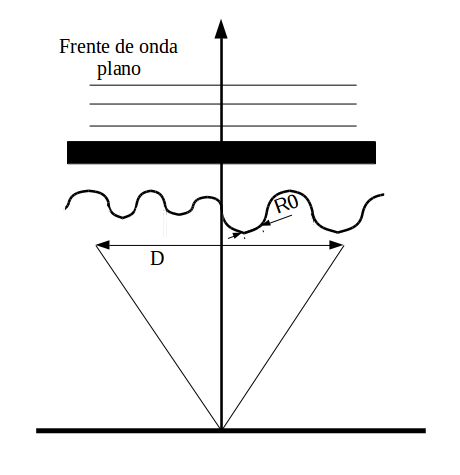
\includegraphics[scale=0.25]{Esquema.png}
					\caption{\label{Img:Esquema}Esquema del sistema simulado para estudiar el efecto Speckle. En la imagen $D$ corresponde al tamaño de la lente o Espejo del telescopi y $R0$ a la aproximación del frente de onda aleatorio en la cuál el frente de onda es constante y se puede aplicar la corrección.}
				\end{figure}

			Para el caso de un foco puntual, si no hubiese cambios en la fase se debería obtener la mancha de Airy. Para el efecto de Speckle se pueden obtener también diferentes aproximaciones a este patrón en función de $D$ y $r_0$:

				\begin{equation}
					\begin{matrix}
						D/r_0 >> 1 & \rightarrow & Imagen \neq Airy
						\\
						D/r_0 << 1 & \rightarrow & Imagen=Airy
					\end{matrix}
				\end{equation}

		\section{Desarrollo Experimental}

			El estudio del efecto Speckle producido por diferencias en la fase del frente de onda se ha realizado mediante una simulación a partir del código \cite{Speckle} escrito por el alumno en el lenguaje Python.

			Para crear cada uno de los espejos o pupilas se ha utilizado una clase llamada Espejo que crea los espejos teniendo en cuenta el tamaño del campo, el tamaño del espejo o pupila, forma del espejo, curvatura e inclinación. La forma utilizada para las puìlas pequeñas ha sido la de un hexágono, ya que ésta te permite poder cubrir todo el espacio sin dejar huecos, la forma del espejo grande ha sido circular En el apéndice \ref{appen:Espejo} se muestra como se ha obtenido la matriz para el espejo grande.

			


		\section{Resultados}

			TEXTO
		
		\section{Discusión}

			TEXT

		\section{Conclusiones}

			TEXTO

	\end{multicols}

%----------------------------------------------------------------------------
%     APPENDIX
%----------------------------------------------------------------------------

\newpage

	    \appendix

		    	\section{Obtención del Espejo}
		    		\label{appen:Espejo}

					Para  $(\sqrt{k^2+j^2}=r_{k,j}) < R$:

						\begin{equation}
							Espejo_{k, j} = 1 \cdot e^{i\cdot crv \cdot r_{k,j}} \cdot e^{i\cdot (tip\cdot r_k + tilt \cdot r_j)}
						\end{equation}
						
					Para $(\sqrt{k^2+j^2}=r_{k,j}) = R$:

						\begin{equation}
							Espejo_{k,j} = 0.5 \cdot e^{i\cdot crv \cdot r_{k,j}} \cdot e^{i\cdot (tip\cdot r_k + tilt \cdot r_j)}
							\label{eq:Espejo}
						\end{equation}	

					Siendo $(k, j)$ las coordenadas $(x, y)$ de la matriz, $r_{k, j}$ el radio de esas coordenadas respecto al centro de la matriz, $R$ el radio del espejo, $crv$ la curvatura, $tip$ la inclinación respecto al eje $X$ y $tilt$ la inclinación respecto al eje $Y$.
	    		
%----------------------------------------------------------------------------
%     BIBLIOGRAPHY
%----------------------------------------------------------------------------

	\bibliographystyle{unsrt}
	\bibliography{biblio}

\end{document}


%----------------------------------------------------------------------------
%            TEMPLATES
%----------------------------------------------------------------------------

%----------------------------------------------------------------------------
%            how to insert an image
%----------------------------------------------------------------------------

%	\begin{figure}[H]
%		\centering
%		\includegraphics[scale= ]{nombre de la imagen.jpg}
%		\caption{\label{Img:widgets}el pie de pagina que le quieras 	poner a la imagen}
%	\end{figure}
 
%----------------------------------------------------------------------------
%            how to insert a table
%----------------------------------------------------------------------------

%	\begin{table}[H]
%		\centering
%		\begin{tabular}{|c|c|c|c|}
%			\hline
%			\centering
%				Altura(h) & Distancia (d) & Elaboracion (e) & Longitud (l) \\
%				($\pm0.5$ mm) & ($\pm0.5$ mm) & ($\pm0.5$ mm) & ($\pm0.5$ mm) \\ \hline
%				 &  &  &  \\ \hline
%				 &  &  &  \\ \hline
%				 &  &  &  \\ \hline
%				 &  &  &  \\ \hline
%				 &  &  &  \\ \hline
%		         &  &  &  \\ \hline
%		\end{tabular}
%		\caption{\label{Tab:widgets}pie de pagina que le quieras poner}
%	\end{table}

%----------------------------------------------------------------------------
%             How to remove the label in equactions
%----------------------------------------------------------------------------

%	\begin{equation*}
%		
%	\end{equation*}

%----------------------------------------------------------------------------
%              How to set bibliography
%----------------------------------------------------------------------------

%\bibliographystyle{unsrt}
%\bibliography{biblio}
%
%Then you have to set a .bib document such as the next template
%
%	@book{nickname,
%	author = {},
%	title = {},
%	edition = {},
%	year = {},
%	volume = {},
%	ISBN = {}
%	}
%
%	@ARTICLE{nickname,
%	author = {},
%	title = {},
%	year = {},
%	volume = {},
%	}


%----------------------------------------------------------------------------
%              END
%----------------------------------------------------------------------------
